\documentclass[a4paper,12pt]{report}

% Paquete para inclusion de graficos.
\usepackage{graphicx}

% Paquete para definir la codificacion del conjunto de caracteres usado
% (latin1 es ISO 8859-1).
\usepackage[latin1]{inputenc}

% Paquete para definir el idioma usado.
\usepackage[spanish]{babel}


% Titulo principal del documento.
\title{TP2: Simulador de Cache}

% Informacion sobre el autor.
\author{	Santiago Alvarez Juli\'a, \textit{Padr\'on Nro. 99522}                     \\
            \normalsize{75.42 Taller de Programaci\'on}                             \\
            \normalsize{Facultad de Ingenier\'ia, Universidad de Buenos Aires}            \\
       }
\date{Septiembre 2018}


\begin{document}

% Inserta el titulo.
\maketitle

% Quita el numero en la primer pagina.
\thispagestyle{empty}

% Crea la tabla de contenidos o indice del informe
\pagenumbering{roman}
\tableofcontents
\newpage
\pagenumbering{arabic}

% Aca arranca el cuerpo del informe
\section{Introducci\'on}

En las siguientes secciones abordar\'e algunos temas claves para la resolucion del programa Simulador de cache. Respecto a la base de programaci\'on de ejercicios anteriores, este difiere en 2 puntos claves :

\begin{itemize}
\item Programaci\'on Orientada a Objetos (POO)
\item Multi Threading
\end{itemize}


\section{Temas Claves}

\subsection{Programaci\'on Orientada a Objetos}

Excepto la funcion main, todo el resto del programa fue dise\~nado en base a objetos que se relacionan entre si. A continuaci\'on har\'e una breve descripci\'on de cada objeto de la aplicaci\'on.

\begin{itemize}

\item Thread: este objecto encapsula la clase std::thread (que representa un hilo de ejecuci\'on). Dentro del m\'etodo start llamo al constructor de inicializaci\'on de std::thread que recibe como par\'ametros un puntero al m\'etodo run de Thread y un puntero al objecto para el cual esta definido el m\'etodo run. Dicho m\'etodo run es virtual puro, por lo tanto Thread es una clase abstracta. Esto permite que cualquier objeto pueda correr en su propio hilo mientras herede de Thread e implemente el m\'etodo run.    

\item FunctorCache: como lo indica su nombre este objecto es un functor, su objetivo es encapsular la funci\'on que debe ejecutarse cuando se lanza un hilo. Esta clase hereda de Thread e implementa el m\'etodo run. Dentro de dicho m\'etodo se parsean los archivos binarios que contienen las direcciones de memoria (1 archivo por hilo). Para cada direcci\'on de memoria se le pregunta al atributo CacheProtected si la direcciones es valida y en caso contrario imprime que es invalida. En el caso positivo, se le vuelve a enviar la direcci\'on a CacheProtected para que la procese. En el caso negativo, se finaliza la ejecuci\'on del hilo.

\item CacheProtected: este objecto encapsula al objecto compartido por todos los hilos Cache, su mutex protector y un mutex mas que protege al std::cerr. El mutex protector de cache es utilizado en un unico metodo, que a su vez es el unico metodo en el cual se podria imprimir por std::cout durante la ejecucion multihilo, por lo tanto prescindo de un mutex que proteja a std::cout en particular. Su objetivo es lockear mutex cuando sea necesario, su comportamiento lo delega completamente al objeto Cache (excepto la validaci\'on de direcciones de memoria). 

\item Cache: es una clase abstracta que tiene como clases derivadas CacheDirect, CacheFifo y CacheLru. Tiene como m\'etodo virtual puro 'proccesMemoryAddress' cuya implementaci\'on depende de las clases derivadas. Esta clase tiene como objetivo permitir el polimorfismo para que las distintas clases de cache hagan su propia implementaci\'on de m\'etodos que dependan del tipo de clase derivada. Para el resto de los m\'etodos cuya implementaci\'on es com\'un a todas las caches, esta se escribe en el .cpp de Cache y as\'i evitar repetici\'on de c\'odigo. An\'alogamente sucede lo mismo con los atributos del objeto, si sus comportamientos son comunes a todas las clases derivadas de Cache, estos se escribe en el .cpp de Cache y se declaren como protegidos para que solo puedan acceder clases hijas.

\item CacheDirect: esta clase es hija de la clase Cache. Utilizo un std::map para simular una cache directa ya que la \'unica condici\'on que se debe cumplir es que la b\'usqueda de tags sea de orden de complejidad menor a n (siendo n la cantidad de elementos que contiene), el m\'etodo 'find' de std::map tiene orden de complejidad log (n).

\item CacheFifo y CacheLru: ambas clases son hijas de la clase Cache. En ambas utilizo un std::map para la b\'usqueda de tags (al igual que en CacheDirect utilizo el m\'etodo 'find'). Para simular la cache asociativa utilizo el std::deque. En ambos utilizo std::deque xq me permite agregar tags al cache en O(1) con el m\'etodo 'pushBack'. En el caso de la CacheFifo tambi\'en es  O(1) reemplazar un bloque cuando se llena la cache con el m\'etodo 'popFront'. \\

En el caso de CacheLru gracias a std::deque agregar un bloque al cache cuando hay un miss y este no esta lleno es O(1) y borrar de la cache el bloque menos usado recientemente tambi\'en es O(1) con el m\'etodo 'popFront'. Cuando hay un hit debe borrarse el bloque viejo que contiene el mismo tag y agregar al principio el bloque nuevo para que tenga sentido usar 'popFront', para realizar ese reemplazo anteriormente almaceno un iterador a cada elemento que agrego al std::deque y lo amaceno en el std::map donde la clave es el tag asociado a dicho iterador.  Por lo tanto quitar un elemento de std::deque con un iterador es O(1), lo que mas cuesta es almacenar el iterador en el map, lo realizo con el operador[], el cual tiene  orden de complejidad log (n).

En ambas implementaciones tambi\'en utilizo el m\'etodo 'size' de std::map para saber si la cache esta llena que seg\'un documentaci\'on es O(1).\\

Me parece importante aclarar que ser\'ia mejor implementar a CacheFifo y CacheLru como clases derivadas de una nueva clase llamada CacheAsociativa que sea abstracta y sea hija de Cache. Como lo aclara su nombre, ambas caches fifo y lru se comportan de la misma manera excepto en la pol\'itica de reemplazo. No lo implemente de tal manera por falta de tiempo.
 
\item Lock: es una encapsulaci\'on RAII de la toma y la liberaci\'on del recurso mutex.


\end{itemize}


\subsection{Multi Threading}

Dentro del main thread se lanzan el resto de los hilos, 1 por cada archivo de direcciones de memoria ya que la informaci\'on que almacenan puede ser procesada independientemente. El programa tiene una critical section que es verificar si dado un tag, este se encuentra en la cache y actuar en funci\'on de eso. Tambi\'en pueden ocurrir race conditions cuando se quiere imprimir por pantalla, ya sea por std::cout o std::cerr porque ambos archivos son compartidos por todos los hilos.

\begin{itemize}

\item Cache : existe una \'unica instancia de Cache y tiene su propio mutex. Ambos elementos est\'an encapsulados en el objeto CacheProtected. Dicho mutex es lockeado solamente cuando hay que procesar un tag, justo despu\'es de verificar si el tag representa una direcci\'on de memoria v\'alida, es decir cuando quiero verificar si dicho tag produce un hit o miss en la cache. Dentro de CacheProtected es lockeado dicho mutex justo antes de llamar al m\'etodo 'proccesMemoryAddress'.

\item Std::cout y std::cerr : antes de lanzar los hilos se abre el archivo de configuraci\'on y se imprime por pantalla est\'andar los datos de la cache y luego de "joinear" los hilos se imprime tambi\'en por salida est\'andar el informe de hits y misses que generaron los archivos de direcciones de memoria en la cache. Ninguna de las anteriores impresiones podr\'ia generar una race condition porque siempre van a suceder cuando solamente el main thread est\'a ejecut\'andose.\\

En cambio cuando se ejecutan los hilos pueden suceder 2 cosas que podr\'ian producir race conditions: una direcci\'on de memoria inv\'alida y en el caso de que la cache tenga el modo debug en true, cada vez que se produce un hit o miss se tendr\'ia que imprimir sin problemas por salida est\'andar lo sucedido. El primer caso tiene como recurso compartido la salida de error est\'andar std::cerr por lo tanto para evitar la race condition CacheProtected tambi\'en almacena un mutex asociado unicamente con std::cerr que es lockeado antes de verificar la validez de la direcci\'on de memoria que se esta procesando. Para el segundo caso se da la situaci\'on particular de que el recurso compartido std::cout esta protegido por el mutex de la cache ya que este es lockeado solamente cuando hay que procesar un tag, justamente la \'unica situaci\'on en la que se podr\'ia producir una race condition (es decir en el m\'etodo 'proccesMemoryAddress' de cache).

\end{itemize}

\section{Diagramas}

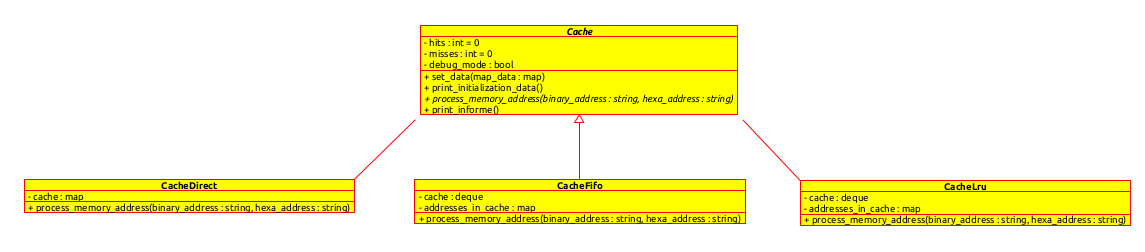
\includegraphics[width=15cm]{diagramaClasesCache.png}

\end{document}